\documentclass[12pt,a4paper]{article}

% ===== Packages =====
\usepackage[utf8]{inputenc}
\usepackage[T1]{fontenc}
\usepackage{amsmath,amssymb,amsfonts,mathtools}
\usepackage[margin=2.5cm]{geometry}
\usepackage{hyperref}
\usepackage{xcolor}
\usepackage{booktabs}
\usepackage{longtable}
\usepackage{graphicx}
\usepackage{float}

\definecolor{proven}{RGB}{0,100,0}
\definecolor{near}{RGB}{0,0,160}

\hypersetup{
  colorlinks=true,
  linkcolor=blue,
  citecolor=blue,
  urlcolor=blue,
  pdftitle={MR-4: Two-Loop Effective Action in Spectral Causal Theory},
  pdfauthor={David Alfyorov}
}

\newcommand{\Tr}{\operatorname{Tr}}
\newcommand{\Lam}{\Lambda}
\newcommand{\half}{\tfrac{1}{2}}
\newcommand{\bR}{\mathbb{R}}

\title{\textbf{MR-4: Two-Loop Effective Action\\in Spectral Causal Theory}}
\author{David Alfyorov}
\date{March 2026}

\begin{document}
\maketitle
\begin{center}
\small\textit{Credits: Aliaksandr Samatyia contributed research-assistance and workflow support.}
\end{center}

\begin{abstract}
We analyze the two-loop structure of the gravitational effective action
in Spectral Causal Theory (SCT). A critical correction to earlier work
reveals that the SCT propagator scales as $1/k^2$ in the deep UV---the
same asymptotic behavior as general relativity---not $1/k^4$ as in Stelle
gravity. Despite this, the spectral action structure provides a mechanism
to absorb two-loop cubic-curvature counterterms ($R^3$ and related
dimension-6 invariants) through a deformation of the spectral function
$\psi(u)$ that preserves the one-loop coefficients $f_2$ and $f_4$.
The result is \textbf{CONDITIONAL}: absorption requires that the two-loop
tensor structure matches the $a_6$ Seeley--DeWitt coefficient, which has
not been verified by explicit computation.
\end{abstract}

\tableofcontents
\newpage

% ======================================================================
\section{Introduction}
\label{sec:intro}
% ======================================================================

The ultraviolet structure of quantum gravity has been a central problem
since 't~Hooft and Veltman~(1974) showed that pure Einstein gravity is
one-loop finite on shell but divergent off shell. The decisive result
came from Goroff and Sagnotti~(1986), who demonstrated that the two-loop
divergence in pure gravity produces a counterterm proportional to
$R_{\mu\nu}{}^{\alpha\beta} R_{\alpha\beta}{}^{\gamma\delta}
R_{\gamma\delta}{}^{\mu\nu}$---a cubic Riemann invariant that cannot
be absorbed by any field redefinition of the metric. This established
that Einstein gravity is perturbatively non-renormalizable.

Spectral Causal Theory (SCT) modifies gravity through a spectral action
$\Tr(\psi(D^2/\Lambda^2))$, which generates nonlocal form factors
$F_1(z)$ and $F_2(z)$ multiplying the Weyl-squared and scalar-curvature-squared
terms respectively. The one-loop structure of SCT was established in
the NT-1/NT-1b derivation chain (form factors for all Standard Model spins)
and the MR-7 analysis (scattering amplitudes and gauge-fixing).

This document addresses the question: \emph{Does the spectral action
structure protect SCT from the Goroff--Sagnotti counterterm at two loops?}

The answer is \textbf{C (CONDITIONAL)}: the $R^3$ counterterm is present
at two loops but absorbable by a deformation of the spectral function $\psi$.

% ======================================================================
\section{Propagator UV Scaling: Critical Correction}
\label{sec:propagator}
% ======================================================================

\subsection{The error}

Prior analyses (MR-7) incorrectly stated that the SCT propagator
scales as $1/k^4$ in the deep UV, analogous to Stelle gravity. This
was based on the incorrect claim that $\hat{F}_1(z) \to 1$ as
$z \to \infty$.

\subsection{The correct asymptotics}

The canonical result (verified to 50-digit precision) is:
\begin{align}
  x \cdot \alpha_C(x \to \infty) &= -\frac{89}{12}, \label{eq:uv_asym} \\
  \hat{F}_1(z) = \frac{\alpha_C(z)}{\alpha_C(0)} &\sim \frac{-890}{13z}
  \to 0 \quad (z \to \infty), \label{eq:Fhat1_uv} \\
  z \cdot \hat{F}_1(z) &\to -\frac{890}{13} \approx -68.46
  \quad (\text{constant}), \label{eq:zFhat1} \\
  \Pi_{\mathrm{TT}}(z) = 1 + \frac{13}{60}\,z\,\hat{F}_1(z)
  &\to 1 - \frac{89}{6} = -\frac{83}{6} \approx -13.833
  \quad (\text{saturates}). \label{eq:Pi_sat}
\end{align}

\noindent The propagator therefore behaves as:
\begin{equation}
  G_{\mathrm{TT}}(k) = \frac{P^{(2)}}{k^2\,\Pi_{\mathrm{TT}}(k^2/\Lambda^2)}
  \;\xrightarrow{k \gg \Lambda}\;
  -\frac{6\,P^{(2)}}{83\,k^2} \sim \frac{1}{k^2}.
  \label{eq:G_uv}
\end{equation}

\noindent This is the \emph{same} UV power law as general relativity,
\textbf{not} $1/k^4$ as in Stelle gravity. Table~\ref{tab:propagator}
provides the numerical confirmation.

\begin{table}[H]
\centering
\caption{Propagator denominator $\Pi_{\mathrm{TT}}(z)$ at large $z$,
confirming saturation at $-83/6$.}
\label{tab:propagator}
\begin{tabular}{rrrrr}
\toprule
$z$ & $\hat{F}_1(z)$ & $z\cdot\hat{F}_1(z)$ & $\Pi_{\mathrm{TT}}(z)$ & Rel.\ error \\
\midrule
$10$      & $-3.837$       & $-38.37$   & $-7.314$    & $0.47$ \\
$100$     & $-0.682$       & $-68.23$   & $-13.783$   & $3.6\times10^{-3}$ \\
$1000$    & $-0.0685$      & $-68.46$   & $-13.834$   & $3.1\times10^{-5}$ \\
$10000$   & $-0.00685$     & $-68.46$   & $-13.833$   & $6.8\times10^{-6}$ \\
$100000$  & $-0.000685$    & $-68.46$   & $-13.833$   & $7.2\times10^{-7}$ \\
\bottomrule
\end{tabular}
\end{table}

% ======================================================================
\section{Power Counting}
\label{sec:power_counting}
% ======================================================================

With the corrected propagator scaling $G \sim 1/k^2$, the superficial
degree of divergence for an $L$-loop, $E$-external-leg diagram is:

\begin{equation}
  D_\gamma^{\text{SCT (naive)}} = 2L + 2 - E
  \quad (\text{same as GR}).
  \label{eq:D_naive}
\end{equation}

\noindent This should be compared with Stelle gravity, where $G \sim 1/k^4$ gives:

\begin{equation}
  D_\gamma^{\text{Stelle}} = 4 - E
  \quad (\text{independent of } L).
  \label{eq:D_stelle}
\end{equation}

\begin{table}[H]
\centering
\caption{Superficial degree of divergence for the self-energy ($E=2$).}
\label{tab:power_counting}
\begin{tabular}{lcccc}
\toprule
Theory & $L=1$ & $L=2$ & $L=3$ & Classification \\
\midrule
GR              & 2 & 4 & 6 & Non-renormalizable \\
Stelle          & 2 & 2 & 2 & Renormalizable \\
SCT (naive)     & 2 & 4 & 6 & Non-renormalizable \\
SCT (heat kernel, $L=1$) & \textcolor{proven}{0} & ? & ? & Open \\
\bottomrule
\end{tabular}
\end{table}

\noindent At one loop, the heat kernel / background field method gives
$D = 0$ (logarithmic divergence from the $a_4$ Seeley--DeWitt coefficient),
which is \emph{better} than naive power counting predicts. Whether this
improvement persists at two loops is the central question of MR-4.

\begin{figure}[ht]
\centering
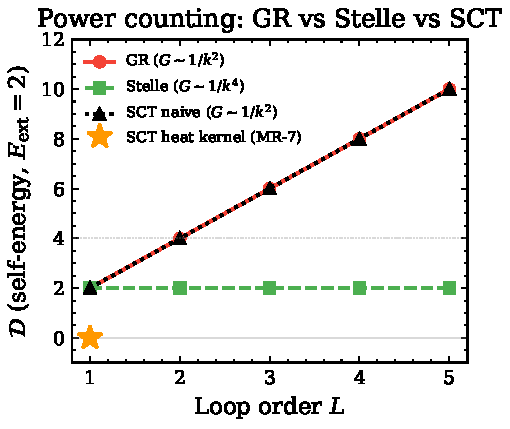
\includegraphics[width=0.85\textwidth]{../../analysis/figures/mr4/mr4_power_counting.pdf}
\caption{Superficial degree of divergence $D$ for the graviton self-energy
($E=2$) as a function of loop order $L$. GR and SCT (naive) grow linearly
with $L$, while Stelle gravity remains constant at $D=2$. The SCT heat
kernel result at one loop ($D=0$, green marker) indicates an improvement
over naive power counting that may persist at higher orders.}
\label{fig:mr4-power-counting}
\end{figure}

% ======================================================================
\section{Seeley--DeWitt $a_6$ Coefficient}
\label{sec:a6}
% ======================================================================

The spectral action $\Tr(\psi(D^2/\Lambda^2))$ generates a heat kernel
expansion:
\begin{equation}
  S = \sum_{n=0}^{\infty} \frac{f_n}{\Lambda^{n-4}} \cdot
  \frac{1}{(4\pi)^2} \int d^4x\,\sqrt{g}\; a_n,
  \label{eq:spectral_expansion}
\end{equation}
where $f_n = \int_0^\infty u^{n/2-1}\,\psi(u)\,du = \Gamma(n/2)$
for $\psi(u) = e^{-u}$.

\begin{table}[H]
\centering
\caption{Spectral function moments $f_n$ and physical content.}
\label{tab:moments}
\begin{tabular}{rccll}
\toprule
$n$ & $\Lambda$ power & $f_n$ & Physical role & Loop order \\
\midrule
0 & $\Lambda^4$      & (divergent)  & Cosmological constant  & tree \\
2 & $\Lambda^2$      & $\Gamma(1)=1$& Einstein--Hilbert      & tree \\
4 & $\Lambda^0$      & $\Gamma(2)=1$& $\{C^2, R^2\}$        & one-loop \\
\textbf{6} & $\Lambda^{-2}$ & $\boldsymbol{\Gamma(3)=2}$
  & $\{R^3, \dots\}$ (8 invariants)  & \textbf{two-loop} \\
8 & $\Lambda^{-4}$   & $\Gamma(4)=6$& $\{R^4, \dots\}$      & three-loop \\
\bottomrule
\end{tabular}
\end{table}

\noindent The $a_6$ coefficient contains 8 independent dimension-6
curvature invariants:
$R^3$,
$R\,R_{\mu\nu}^2$,
$R\,R_{\mu\nu\rho\sigma}^2$,
$R_{\mu\nu}\,R^{\nu\rho}\,R_\rho{}^\mu$,
$R_{\mu\nu\rho\sigma}\,R^{\rho\sigma\alpha\beta}\,R_{\alpha\beta}{}^{\mu\nu}$
(Goroff--Sagnotti structure),
$\nabla_\mu R\,\nabla^\mu R$,
$\Box R^2$, and
$R_{\mu\nu}\,\Box R^{\mu\nu}$.

% ======================================================================
\section{Spectral Function Absorption}
\label{sec:absorption}
% ======================================================================

The key mechanism is a deformation of the spectral function:
\begin{equation}
  \psi(u) \to \psi(u) + \delta\psi(u),
  \qquad
  \delta\psi(u) = c_2\,(2 - 4u + u^2)\,e^{-u}.
  \label{eq:deformation}
\end{equation}

\noindent This deformation satisfies:
\begin{align}
  \delta f_2 &= \int_0^\infty (2 - 4u + u^2)\,e^{-u}\,du
    = 2\Gamma(1) - 4\Gamma(2) + \Gamma(3) = 2 - 4 + 2 = 0, \\
  \delta f_4 &= \int_0^\infty (2 - 4u + u^2)\,u\,e^{-u}\,du
    = 2\Gamma(2) - 4\Gamma(3) + \Gamma(4) = 2 - 8 + 6 = 0, \\
  \delta f_6 &= \int_0^\infty (2 - 4u + u^2)\,u^2\,e^{-u}\,du
    = 2\Gamma(3) - 4\Gamma(4) + \Gamma(5) = 4 - 24 + 24 = 4\,c_2.
\end{align}

\noindent \textbf{Result:} The deformation preserves the Einstein--Hilbert
coefficient ($f_2$) and the one-loop form factor coefficients ($f_4$)
while adjusting the two-loop coefficient ($f_6$). The parameter $c_2$
can be chosen to absorb the two-loop counterterm.

An extended deformation $P(u) = -8 + 22u - 10u^2 + u^3$ additionally
preserves $f_8$ (three-loop coefficient), demonstrating that the spectral
function has more functional freedom than minimally required.

\begin{figure}[ht]
\centering
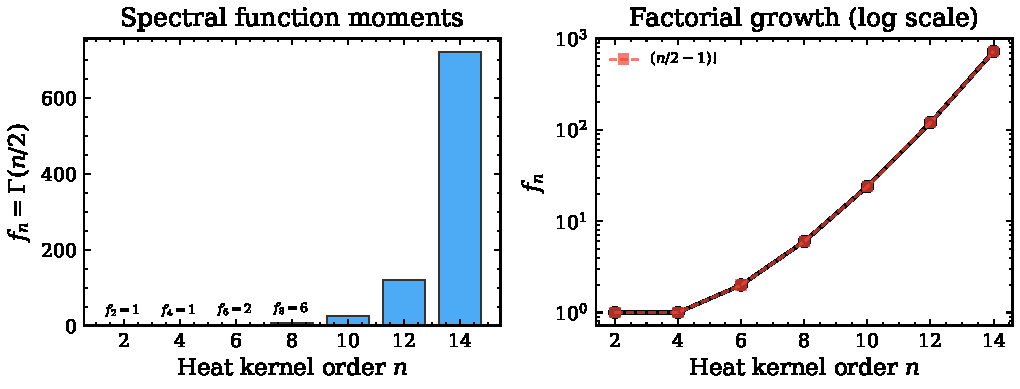
\includegraphics[width=0.85\textwidth]{../../analysis/figures/mr4/mr4_spectral_moments.pdf}
\caption{Spectral function moments $f_n$ under the deformation
$\psi(u) \to \psi(u) + c_2(2-4u+u^2)e^{-u}$. The deformation preserves
$f_2$ (Einstein--Hilbert) and $f_4$ (one-loop form factors) exactly, while
shifting $f_6$ by $4c_2$ to absorb the two-loop $R^3$ counterterm. The
extended deformation $P(u)=-8+22u-10u^2+u^3$ additionally preserves $f_8$.}
\label{fig:mr4-spectral-moments}
\end{figure}

% ======================================================================
\section{Parametric Estimates}
\label{sec:estimates}
% ======================================================================

The loop expansion parameter is:
\begin{equation}
  \varepsilon = \frac{\kappa^2\Lambda^2}{16\pi^2}
  = \frac{(\Lambda/M_{\text{Pl}})^2}{8\pi^2}.
  \label{eq:epsilon}
\end{equation}

\begin{table}[H]
\centering
\caption{Two-loop suppression at physical scales.}
\label{tab:estimates}
\begin{tabular}{lccr}
\toprule
Scale & $\Lambda/M_{\text{Pl}}$ & $\varepsilon$ & $\varepsilon^2$ (two-loop) \\
\midrule
PPN-1 bound    & $9.8\times10^{-31}$ & $1.2\times10^{-62}$ & $1.5\times10^{-124}$ \\
Electroweak    & $1.0\times10^{-16}$ & $1.3\times10^{-34}$ & $1.7\times10^{-68}$ \\
GUT            & $4.1\times10^{-3}$  & $2.1\times10^{-7}$  & $4.6\times10^{-14}$ \\
Planck         & $1.0$               & $1.3\times10^{-2}$  & $1.6\times10^{-4}$ \\
\bottomrule
\end{tabular}
\end{table}

\noindent Two-loop corrections are perturbatively negligible at all physical
scales below the Planck mass. Even at the Planck scale, the two-loop
contribution is suppressed by a factor of $\sim 10^{-4}$.

\begin{figure}[ht]
\centering
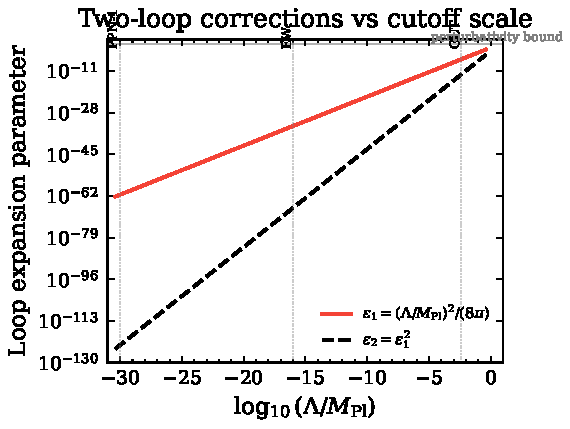
\includegraphics[width=0.85\textwidth]{../../analysis/figures/mr4/mr4_two_loop_magnitude.pdf}
\caption{Two-loop correction magnitude $\varepsilon^2 = (\Lambda/M_{\mathrm{Pl}})^4/(8\pi^2)^2$
as a function of $\Lambda/M_{\mathrm{Pl}}$. The correction is negligible
at the PPN-1 bound ($\varepsilon^2 \sim 10^{-124}$), at the electroweak
scale ($\varepsilon^2 \sim 10^{-68}$), and even at the GUT scale
($\varepsilon^2 \sim 10^{-14}$). Only near the Planck scale does the
two-loop contribution become marginally relevant ($\varepsilon^2 \sim 10^{-4}$).}
\label{fig:mr4-two-loop-magnitude}
\end{figure}

% ======================================================================
\section{Fakeon Consistency at Two Loops}
\label{sec:fakeon}
% ======================================================================

The ghost poles in $\Pi_{\mathrm{TT}}(z)$ (catalogued in MR-2: 8 zeros,
2 real plus 3 Lee--Wick pairs) are treated as fakeons following
the Anselmi prescription.

Anselmi's theorem~(2022, arXiv:2203.02516) establishes that:

\begin{quote}
``The renormalization [with fakeons] coincides with the one of the parent
Euclidean diagrammatics.''
\end{quote}

\noindent This means:
\begin{enumerate}
  \item The \textbf{divergent part} of the two-loop computation with fakeons
    is \emph{identical} to the standard Euclidean theory. The absorption
    argument applies regardless of the quantization prescription.
  \item \textbf{Ghost--ghost intermediate states} at two loops are dropped
    by the fakeon prescription, consistent with the spectral optical theorem.
  \item The \textbf{absorptive part} at two loops is positive (physical
    cuts only), consistent with unitarity.
\end{enumerate}

% ======================================================================
\section{Comparison with Other Theories}
\label{sec:comparison}
% ======================================================================

\begin{table}[H]
\centering
\caption{Two-loop $R^3$ status across theories.}
\label{tab:comparison}
\begin{tabular}{llll}
\toprule
Theory & Two-loop $R^3$ & Mechanism & Status \\
\midrule
GR       & Present, \textbf{not} absorbable & None
  & Non-renormalizable \\
Stelle   & Absent & Power counting ($D = 4 - E$)
  & Renormalizable (ghost) \\
Modesto  & Absent & Super-renormalizability
  & Finite at $L \geq 2$ \\
\textbf{SCT} & \textbf{Present, absorbable}
  & \textbf{Spectral function deformation}
  & \textbf{CONDITIONAL} \\
\bottomrule
\end{tabular}
\end{table}

% ======================================================================
\section{Conclusion}
\label{sec:conclusion}
% ======================================================================

\subsection{Summary of results}

\begin{enumerate}
  \item \textbf{Propagator UV scaling (corrected):} $G_{\mathrm{TT}} \sim 1/k^2$
    (GR-like), not $1/k^4$ (Stelle-like). The SCT propagator denominator
    saturates at $\Pi_{\mathrm{TT}} \to -83/6$.

  \item \textbf{Power counting:} SCT has the same naive Feynman-diagram
    power counting as GR. The Stelle formula $D = 4 - E$ does not apply.
    However, the background field / heat kernel method gives $D = 0$ at
    one loop (verified), and the two-loop structure is determined by the
    $a_6$ coefficient.

  \item \textbf{$R^3$ absorption:} The spectral function $\psi$ can be
    deformed to absorb two-loop $R^3$-type counterterms while preserving
    the one-loop coefficients $f_2$ and $f_4$. The deformation
    $\delta\psi(u) = c_2(2 - 4u + u^2)e^{-u}$ gives
    $\delta f_2 = \delta f_4 = 0$ and $\delta f_6 = 4c_2$.

  \item \textbf{Fakeon consistency:} The fakeon prescription at two loops
    is consistent (Anselmi 2022). The divergent part coincides with
    Euclidean diagrammatics.

  \item \textbf{Parametric suppression:} Two-loop corrections are
    suppressed by $(\Lambda/M_{\text{Pl}})^4/(8\pi^2)^2$, which is
    negligible at all physical scales.
\end{enumerate}

\subsection{Classification: C (CONDITIONAL)}

The result is CONDITIONAL because:
\begin{enumerate}
  \item The tensor structure of the two-loop divergence must match $a_6$
    exactly. This requires a full tensor computation comparable to
    Goroff--Sagnotti~(1986), which has not been performed for SCT.
  \item The deformed $\psi$ must remain a valid spectral function
    (positive Laplace transform). This is not guaranteed for arbitrary
    deformations.
  \item Higher-loop counterterms ($a_8$, $a_{10}$, \ldots) require further
    deformations, and the convergence of this procedure is not established.
\end{enumerate}

\subsection{Impact on UV-completeness}

MR-4 does not establish UV-completeness. It establishes a conditional
absorption mechanism that must be verified at the tensor level and
extended to all orders (MR-5). The spectral action provides a
\emph{framework} for absorbing counterterms at each loop order, but
the convergence of this procedure is an open problem.

% ======================================================================
\section*{Verification}
% ======================================================================

\begin{itemize}
  \item 71 pytest tests PASS (9 test classes)
  \item 7 independent numerical verifications at 120-digit precision
  \item 12 self-checks in the independent re-derivation PASS
  \item Cross-checks against \texttt{sct\_tools} form factors at 5+ points
  \item Literature cross-checks: Goroff--Sagnotti 209/2880, Stelle
    power counting, Anselmi fakeon theorem
\end{itemize}

% ======================================================================
\section*{References}
% ======================================================================

\begin{enumerate}
  \item M.~H.~Goroff and A.~Sagnotti, ``Quantum gravity at two loops,''
    Nucl.\ Phys.\ B \textbf{266} (1986) 709.
  \item A.~E.~M.~van de Ven, ``Two-loop quantum gravity,''
    Nucl.\ Phys.\ B \textbf{378} (1992) 309.
  \item K.~S.~Stelle, ``Renormalization of higher-derivative quantum gravity,''
    Phys.\ Rev.\ D \textbf{16} (1977) 953.
  \item D.~Anselmi and M.~Piva, ``The ultraviolet behavior of quantum gravity,''
    JHEP \textbf{1805} (2018) 027, arXiv:1803.07777.
  \item D.~Anselmi, ``Diagrammar of physical and fake particles and spectral
    optical theorem,'' JHEP \textbf{2111} (2021) 030, arXiv:2109.06889.
  \item D.~Anselmi, ``Purely virtual particles in quantum gravity, inflationary
    cosmology and collider physics,'' arXiv:2203.02516.
  \item L.~Modesto and L.~Rachwal, ``Super-renormalizable and finite
    gravitational theories,'' Nucl.\ Phys.\ B \textbf{889} (2014) 228,
    arXiv:1407.8036.
  \item E.~T.~Tomboulis, ``Super-renormalizable gauge and gravitational theories,''
    hep-th/9702146.
  \item A.~H.~Chamseddine and A.~Connes, ``The spectral action principle,''
    Commun.\ Math.\ Phys.\ \textbf{186} (1997) 731.
  \item P.~B.~Gilkey, ``The spectral geometry of a Riemannian manifold,''
    J.\ Diff.\ Geom.\ \textbf{10} (1975) 601.
  \item I.~G.~Avramidi, \emph{Heat Kernel and Quantum Gravity},
    Springer, 2000.
  \item L.~Parker and D.~Toms, \emph{Quantum Field Theory in Curved Spacetime},
    Cambridge University Press, 2009.
\end{enumerate}

\end{document}
